\subsection{Taylor Polynomial}\label{subsec-taylor-polynomial}

Under certain conditions on $f$ near $x_0$ we will be able to find for any $\varepsilon>0$
a polynomial $p$ such that $f(x_0)=p(x_0)+R(x_0)$ where $R$ denotes the remainder ($\abs{R(x_0)}<\varepsilon$),
accounting for the inaccuracy of the approximation near $x_0$.

\begin{lemma}\label{lemma-polynomial-derivatives}
	Let $p_n(x)$ be a polynomial of degree $n$ of the function $f$ at the point $x$,
	such that
	\begin{equation}\label{eq-polynomial-derivatives:1}
		p_n(x) = \sum_{k=0}^n \beta_k x^k
	\end{equation}
	Then for any $k\in[0,n]$,
	\begin{equation}\label{eq-polynomial-derivatives:2}
		p_n^{(k)}(x) = \beta_k k!
	\end{equation}
\end{lemma}

\begin{proof}
	Of \pref{lemma}{lemma-polynomial-derivatives}.
	\begin{flushleft}
		If we differentiate the polynomial $p_n(x)$ $k$-times, then
		\begin{itemize}
			\item all terms of degree less than $k$ are zero
			\item for the $k$'th term ($\beta_k x^k$) we get $\beta_k k!$
			\item all terms of degree higher than $k$ disappear at $x=0$
		\end{itemize}
	\end{flushleft}
\end{proof}

\begin{rem}
	By the previous \pref{lemma}{lemma-polynomial-derivatives}, define the coefficients as
	\begin{equation*}
		\beta_k = \frac{p_n^{(k)}(x)}{k!}
	\end{equation*}
\end{rem}

\begin{definition}\label{def-taylor-polynomial}
	Let $n\in\mathbb{N}$ and $f$ be a $n$-times differentiable function at the point
	$x_0\in\domain{f}$. We call \cite[p.214]{wuest2009}
	\begin{equation}\label{eq-taylor-polynomial}
		p_n(f,x_0)(x) \defines \sum_{k=0}^n \frac{f^{(k)}(x_0)}{k!}(x-x_0)^k \qquad(x\in\mathbb{R})
	\end{equation}
	the Taylor polynomial of degree $n$ of the function $f$ at the point $x_0$.
\end{definition}

\begin{definition}\label{def-maclaurin-polynomial}
	The Taylor polynomial introduced in \pref{definition}{def-taylor-polynomial}
	is called Maclaurin polynomial, if $x_0=0$. So,
	\begin{equation}\label{eq-maclaurin-polynomial}
		p_n(f,0)(x) \defines \sum_{k=0}^n \frac{f^{(k)}(0)}{k!}x^k
	\end{equation}
\end{definition}

\begin{exm}\label{exm-sin-taylor-series}
	Find the Maclaurin polynomial for the function $f(x)=\sin(x)$ of degree $3$.
	\begin{flushleft}
		\textbf{Answer}: Since the Maclaurin polynomial evaluates at $x_0=0$,
		we find that
		\begin{align*}
			 & f(x)=\sin(x) \implies f(0)=0         \\
			 & f'(x)=\cos(x) \implies f'(0)=1       \\
			 & f''(x)=-\sin(x) \implies f''(0)=0    \\
			 & f'''(x)=-\cos(x) \implies f'''(0)=-1 \\
		\end{align*}
		So the polynomial is
		\begin{align*}
			p_3(\sin,0) & = f(0) + f'(0)x + \frac{f''(0)}{2!}x^2 + \frac{f'''(0)}{3!}x^3 \\
			            & = x - \frac{x^3}{3!}
		\end{align*}
	\end{flushleft}
	See \pref{figure}{sketch:taylor-polynomial:1} for an comparison between the
	original function and its approximation using the Maclaurin expansion.
	\begin{figure}[ht!]
		\centering
		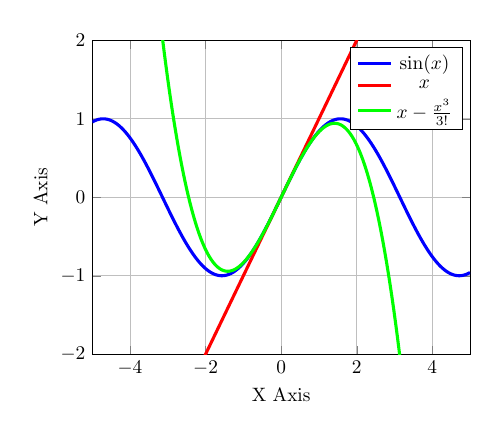
\begin{tikzpicture}[scale=0.7]
			\begin{axis}[
					xmax=5,
					xmin=-5,
					ymax=2,
					ymin=-2,
					samples=1000,
					grid=major,
					xlabel={X Axis},
					ylabel={Y Axis}]
				\addplot[blue, ultra thick,domain=-5:5]{sin(deg(x))};
				\addplot[red, ultra thick,domain=-5:5]{x};
				\addplot[green, ultra thick,domain=-5:5]{x-(x^3/3!)};
				\legend{$\sin(x)$,$x$,$x-\frac{x^3}{3!}$}
			\end{axis}
		\end{tikzpicture}
		\caption{Plot of the Taylor expansion for the function $\sin(x)$}
		\label{sketch:taylor-polynomial:1}
	\end{figure}
\end{exm}

\begin{exm}\label{exm-ln-taylor-series}
	Find the Maclaurin polynomial for the function $f(x)=\ln(x+1)$ of degree $n$.
	\begin{flushleft}
		\textbf{Answer}: Since the Maclaurin polynomial evaluates at $x_0=0$,
		we find that
		\begin{align*}
			 & f(x)=\ln(x+1) \implies f(0)=0                 \\
			 & f'(x)=\frac{1}{x+1} \implies f'(0)=1          \\
			 & f''(x)=-\frac{1}{(x+1)^2} \implies f''(0)=-1  \\
			 & f'''(x)=\frac{2}{(x+1)^3} \implies f'''(0)=-2 \\
		\end{align*}
		After a while it becomes easier to see that there is a pattern to this equation:
		\begin{align*}
			p_n(\ln(x+1),0) & = f(0) + f'(0)x + \frac{f''(0)}{2!}x^2 + \frac{f'''(0)}{3!}x^3 + \cdots + \frac{f^{(n)}(0)}{n!}x^n \\
			                & = x - \frac{x^2}{2} + \frac{x^3}{3} + \cdots + (-1)^{n+1}\frac{x^n}{n}                             \\
			                & = \sum_{k=1}^n (-1)^{k+1}\frac{x^k}{k}
		\end{align*}
	\end{flushleft}
\end{exm}

\begin{thm}\label{thm-taylor-lagrange-remainder-theorem}
	Let $f$ be a $n+1$-times differentiable function in a neighborhood of $x_0$,
	and let $x_0$ be a in that neighborhood. Then by Lagrange's remainder theorem
	there exists a point $\xi$ between $x_0$ and $x$ such that
	\begin{equation}\label{eq-taylor-lagrange-remainder-theorem}
		f(x) = p_n(f,x_0)(x) + \underbrace{\frac{f^{(n+1)}(\xi)}{(n+1)!}(x-x_0)^{n+1}}_{R_n(x)}
	\end{equation}
	where the error incurred by approximating $f$ is denoted by $R_n(x)$ and is
	called the remainder in Lagrange form.
\end{thm}

\begin{rem}
	For $n=0$ we get
	\begin{align*}
		f(x)             & = f(x_0) + f'(\xi)(x-x_0)   \\
		\implies f'(\xi) & = \frac{f(x)-f(x_0)}{x-x_0}
	\end{align*}
	So \hyperref[thm-mean-value-theorem]{the mean value theorem} is a special case
	of Lagrange's remainder theorem.
\end{rem}

\begin{exm}\label{exm-exp-taylor-series}
	The Maclaurin series of the exponential function can be easily found as
	\begin{equation*}
		p_n(\exp(x),0) = \sum_{k=0}^n \frac{x^k}{k!}
	\end{equation*}
	so we can approximate $f(x)=\exp(x)$ with a Taylor polynomial of degree $5$, \textit{i.e.}
	\begin{equation*}
		e^x = p_n(\exp(x),0) + R_n(x)
	\end{equation*}
	Now suppose we require $(\star)$ the remainder in Lagrange form to have at most an
	inaccuracy of $\tfrac{1}{100}$. Then there exists an $0<\xi<1$ and we can roughly
	estimate inaccuracy by
	\begin{align*}
		\abs{R_n(x)} & = \abs[\bigg]{\frac{e^\xi}{(n+1)!}}              \\
		             & = \frac{e^\xi}{(n+1)!}                           \\
		             & < \frac{e}{(n+1)!}                               \\
		             & < \frac{3}{(n+1)!}                               \\
		             & < \frac{1}{100}                     &  & (\star)
	\end{align*}
	Turns out that for $n=5$ the last inequality $(\star)$ holds. In fact, this
	estimation's inaccuracy was already found in the previous step to be $\tfrac{3}{6!}=\tfrac{1}{240}$.
\end{exm}

\begin{thm}\label{thm-infinite-taylor-lagrange-remainder-theorem}
	Let $f$ be a function differentiable infinitely many times in a neighborhood of $x_0$.
	Then there exists a constant $K$ such that for all $n\in\mathbb{N}$,
	\begin{equation}\label{eq-infinite-taylor-lagrange-remainder-theorem}
		\abs{f^{(n)}(x)} \leq K \implies R_n(x) \tolim{n}{\infty} 0
	\end{equation}
\end{thm}
